\documentclass[12pt]{article}
\usepackage[margin=1in]{geometry} 
\usepackage[usenames,dvipsnames]{xcolor}
\usepackage{amsmath,amsthm,amssymb,amsfonts}
\usepackage{ulem}
\usepackage{graphicx}
\usepackage{datetime}
\usepackage{float}
\usepackage{tikz}
\usetikzlibrary{calc, intersections}
\usepackage{hyperref}  % always last
\newcommand{\N}{\mathbb{N}}
\newcommand{\Z}{\mathbb{Z}}
\newcommand{\Q}{\mathbb{Q}}
\newenvironment{problem}[2][Problem]{\begin{trivlist}
\item[\hskip \labelsep {\bfseries #1}\hskip \labelsep {\bfseries #2.}]}{\end{trivlist}}

\begin{document}
\pagenumbering{gobble}  % <-- here, not in preamble

\title{MA$\Theta$ Competition Team HW Set 15}
\author{Anders Christensen, Minjoo Kim}
\date{Due April 8, 2026}
\maketitle
\thispagestyle{empty}
\begin{problem}{1}
  State the definition of a rigid transformation.
\end{problem}

\begin{problem}{2}
  For how many of the following types of quadrilaterals does there exist a point in the plane of a quadrilateral that is equidistant from all four vertices of the quadrilateral?
  \begin{enumerate}
    \item A square
    \item A rectange that is not a square
    \item A rhombus that is not a square
    \item A parallelogram that is not a rectangle or a rhombus
    \item An isosceles trapezoid that is not a parallelogram
  \end{enumerate}
\end{problem}

\begin{problem}{3}
Jiwu is throwing a very elastic baseball to Anders, who is 50 meters away from him. The baseball bounces off the ground at some point in its trajectory and reaches Anders's hand. Given that Jiwu is 1.80 meters tall, and Anders is 1.85 meters tall, and both throw/receive the ball at head level, what is the minimum path length of the ball's motion?

\begin{problem}{5}
  Isosceles $\triangle ABC$ has a right angle at $C$. Point $P$ is inside $\triangle ABC$, such that $PA=11$, $PB=7$, and $PC=6$. Legs $\overline{AC}$ and $\overline{BC}$ have length $s=\sqrt{a+b\sqrt{2}}$, where $a$ and $b$ are positive integers. What is $a+b$?
\end{problem}
\begin{figure}[H]
\centering
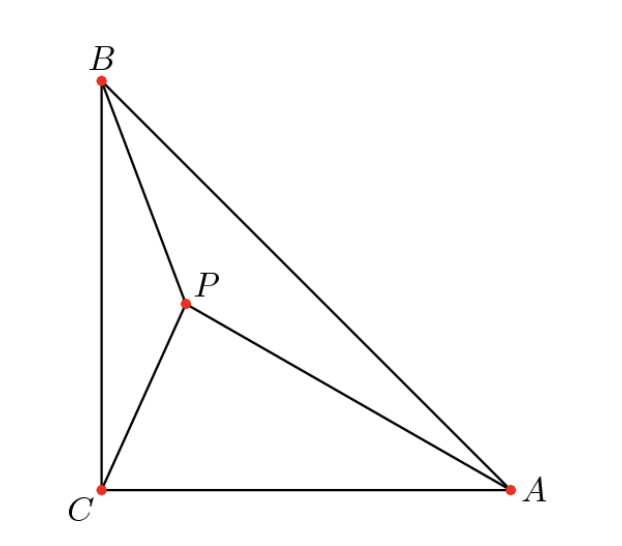
\includegraphics[scale=0.3]{MATHW15-5.png}
\end{figure}
\end{document}
